\chapter{Integration on Manifolds}
Let $M^n$ be an oriented $n$-dimensional smooth manifold. We define an integral
\begin{align*}
  \int_M: \Omega^n_c(M^n)\to \RR
\end{align*}

on the vector space of differential $n$-forms with compact support. Next we shall
consider integration on subsets of $M^n$, and Stokes' theorem will be proved.
Finally we calculate $H^n (M^n)$ for an arbitrary orientable compact connected
smooth manifold $M^n$.

In the special case where $M^n = \RR^n$ (with the standard orientation) we can write
$\omega\in\Omega^n_c(\RR^n)$ in the form 
\begin{align*}
  \omega = f(x)\dd x_1\wedge\cdots\wedge\dd x_n,
\end{align*}

where $f\in C^\infty(\RR^n, \RR)$ has compact support. We then define 
\begin{align*}
  \int_{\RR^n}^{}{f(x)\dd x_1\wedge\cdots\wedge\dd x_n }
  = \int_{\RR^n} f(x)\dd \mu_n
\end{align*}

where $\dd\mu_n$ is the usual Lebesgue measure on $\RR^n$. The same definition can be used
when $\omega\in\Omega^n_c(V)$ for an open set $V\sseq\RR^n$, since $\omega$ and $f$ are smoothly 
extendable to the whole of $\RR^n$ by setting them equal to 0 on $\RR^n-\R{supp}_V(\omega)$.


\begin{lemma}\label{lemma:10-1}
  Let $\phi:V\to W$ be a diffeomorphism between open subsets $V$ and $W$ of $\RR^n$, and 
  assume that we the Jacobi determinant $\det (D_x\phi)$ is of constant sign $\delta=\pm 1$
  for $x\in V$. For $\omega\in \Omega^n_c(W)$ we have that 
  \begin{align*}
    \int_V \phi^*(\omega) = \delta\cdot\int_W \omega.
  \end{align*}
\end{lemma}

\begin{proof}
  If $\omega$ is written in the form 
  \begin{align*}
    \omega = f(x)\dd x_1\wedge\cdots\wedge\dd x_n
  \end{align*}
  with $f\in C_c^\infty(W, \RR)$, it follows from Example \ref{example:3-13}.(ii) that
  \begin{align*}
    \phi^*(\omega)
    & = f(\phi(x))\det(D_x\phi)\dd x_1\wedge\cdots\wedge\dd x_n\\ 
    & = \delta f(\phi(x))|\det(D_x\phi)|\dd x_1\wedge\cdots\wedge\dd x_n.
  \end{align*}

  The assertion follows from the transformation theorem for integrals which states that
  \begin{align*}
    \int_W f(x)\dd\mu_n 
    = \int_V f(\phi(x))|\det(D_x\phi)|\dd\mu_n.
  \end{align*}
\end{proof}

\begin{proposition}\label{prop:10-2}
  For an arbitrary oriented n-dimensional smooth manifold $M^n$ there exists a unique linear map
  \begin{align*}
    \int_M: \Omega^n_c(M^n)\to \RR
  \end{align*}
  with the following properties: If $\omega\in\Omega_c^n(M^n)$ has support contained in $U$, 
  where $(U, h)$ is a positively oriented $C^\infty$-chart, then 
  \begin{align}\label{eq:10-1}
    \int_M \omega = \int_{h(U)} h^{-1}(\omega)^*.
  \end{align}
\end{proposition}

\begin{proof}
  First consider $\omega\in \Omega^n_c(M^n)$ with ``small'' support, i.e. such that $\supp_M(\omega)$
is contained in a coordinate patch. Then $(U, h)$ can be chosen as above and
the integral is determined by \eqref{eq:10-1}. We must show that the right-hand side is
independent of the choice of chart. Assume that $(\tilde{U}, \tilde h)$ is another positively
oriented $C^\infty$-chart with $\supp_M(\omega)\sseq \tilde{U}$.

The diffeomorphism $\phi:V\to W$ from $V=h(U\cap \tilde{U})$ to $W=\tilde{h}(U\cap \tilde{U})$ given 
by $\phi=\tilde{h}\circ h^{-1}$ has everywhere positive Jacobi determinant. Since 
\begin{align*}
  \supp_{h(U)}((h^{-1})^*(\omega))\sseq V, && 
  \supp_{\tilde{h}(\tilde{U})}((\tilde{h}^{-1})^*(\omega))\sseq W,
\end{align*}
and $\phi^*(\tilde{h}^{-1})^*(\omega) = (h^{-1})^*(\omega)$, Lemma \ref{lemma:10-1} shows that 
\begin{align*}
  \int_{h(u)} (h^{-1})^*(\omega) = \int_{\tilde{h}(\tilde{U})} (\tilde{h}^{-1})^*(\omega).
\end{align*}
So for $\omega\in\Omega_c^n(M)$ with ``small'' support the integral defined by \eqref{eq:10-1} is independent
of the chart.

Now choose a smooth partition of unity $(\rho_\alpha)_{\alpha\in A}$ on $M$ subordinate to an 
oriented $C^\infty$-atlas on $M$. For $\omega\in\Omega_c^n(M)$ we have that 
\begin{align*}
  \omega = \sum_{\alpha\in A} \rho_\alpha\omega,
\end{align*}

where every term $\rho_\alpha\omega\in\Omega^n_c(M)$ has ``small'' support, and where only 
finitly many terms are non-zero. We define 
\begin{align*}
  I(\omega) = \sum_{\alpha\in A} \int_M \rho_\alpha\omega,
\end{align*}

where the term associated to $\alpha\in A$ is given by \eqref{eq:10-1}, applied to a $U_\alpha$ with
$\supp_M(\rho_\alpha)\sseq U_\alpha$. It is obvious that $I$ is a linear operator on $\Omega^n_c(M)$. If, in
particular, $\supp_M(\omega)\sseq U$, where $(U, h)$ is a positively oriented $C^\infty$-chart, the
terms of the sum can be calculated by \eqref{eq:10-1}, applied to $(U, h)$. This yields
\begin{align*}
  I(\omega) = \int_M \omega,
\end{align*}

which shows that $I$ is a linear operator with the desired properties. Uniqueness
follows analogously.
\end{proof}

\begin{lemma}\label{lemma:10-3}\;\par 
  \begin{enumerate}[(i)]
    \item $\int_M\omega$ changes sign when the orientation of $M^n$ is reversed.
    \item If $\omega\in\Omega^n_c(M^n)$ has support contained in an open set $W=\subset M^n$, then 
      \begin{align*}
        \int_M\omega = \int_W\omega,
      \end{align*}
      where $W$ is the orientation induced by $M$.
    \item If $\phi:N^n\to M^n$ is an orientation persevering diffeomorphism, then we have that 
      \begin{align*}
        \int_M\omega = 
        \int_N\phi^*(\omega)
      \end{align*}
      for $\omega\in\Omega^n_c(M)$.
  \end{enumerate}
\end{lemma}

\begin{proof}
  By a partition of unity, we can restrict ourselves to the case where
$\supp_M(\omega)$ is contained in a coordinate patch. All three properties are now easy
consequences of Lemma \ref{lemma:10-1} and \eqref{eq:10-1}.
\end{proof}

\begin{remark}\label{remark:10-4}
  In the above we could have considered integrals of continuous
  $n$-forms with compact support on $M^n$. If the orientation of $M$ is given by the
  orientation form $\sigma\in\Omega^n(M)$, a continuous $n$-form can be written uniquely as
  $f\sigma$, where $f\in C^0(M, \RR)$. The support of $f\sigma$ is equal to the support of $f$. The
  integral of \eqref{eq:10-1} extended to continuous $n$-forms gives rise to a linear operator
  \begin{align*}
    I_\sigma: C^n_c(M, \RR)\to \RR; && 
    I_\sigma(f) = \int_M f\sigma.
  \end{align*}
  This linear operator is positive, i.e. $I_\sigma(f)\ge 0$ for $f\ge 0$. By a partition of unity 
  it is sufficient to show this when $\supp(f)\sseq U$, where $(U, h)$ is a positive oriented $C^\infty$-chart.
  Then we have that 
  \begin{align*}
    I_\sigma(f) = \int_{h(U)} f\circ h^{-1}(x)\phi(x)\dd \mu_n,
  \end{align*}
  where $\phi$ is determined by $(h^{-1})^*(\sigma) = \phi(x)\dd x_1\wedge\cdots\wedge\dd x_n$. Since 
  $\phi$ is positive we get $I_\sigma(f)\ge 0$.

  According to Riesz's representation theorem (see for instance chapter 2 of [Rudin])
  $I_\sigma$ determines a positive measure $\mu_\sigma$ on $M$ which satisfies
  \begin{align*}
    \int_M f(x)\dd\mu_\sigma = \int_M f\sigma, \qquad f\in C^n_c(M, \RR).
  \end{align*}
  The entire Lebesgue integration machinery now becomes available, but we shall
  use only very little of it in the following.

  If $M^n$ is an oriented Riemannian manifold, the volume form $\R{vol}_M$ will determine
  a measure $\mu_M$ on $M^n$ analogous to the Lebesgue measure on $\RR^N$. For a compact
  set $K$ the volume of $K$ can be defined by
  \begin{align*}
    \R{vol}(K) = \int_K \R{vol}_M \in \RR.
  \end{align*}
\end{remark}

\begin{definition}\label{def:10-5}
  Let $M^n$ be a smooth manifold. A subset $N\sseq M^n$ is called a
domain with smooth boundary or a codimension zero submanifold with boundary,
if for every $p\in M$ there exists a $C^\infty$-chart $(U, h)$ around $p$, such that
\begin{align}\label{eq:10-2}
  h(U\cap N) = h(U)\cap \RR^n_-.
\end{align}
where $\RR^n_- = \{(x_1, \cdots x_n)\in\RR^n\mid x_1\le 0\}$. 
\end{definition}

Note that \eqref{eq:10-2} is automatically satisfied when $p$ is an interior or an exterior point
of $N$ (one can choose $(U, h)$ with $p\in U$, such that $h(U)$ is contained in an open
half-space in IRn defined by either $x_1 < 0$ or $x_1 > 0$). If $p$ is a boundary point of
$N$ then $h(p)$ has first coordinate equal to zero. Let $(U, h)$ and $(V, k)$ be smooth
charts around a boundary point $p\in \partial N$. The resulting transition diffeomorphism
\begin{align*}
  \phi = k\circ h^{-1}: h(U\cap V)\to k(U\cap V)
\end{align*}

induces a map 
\begin{align*}
  h(U\cap V)\cap \RR^n_- \to k(U\cap V)\cap \RR^n_-,
\end{align*}

which restricts to a diffeomorphism
\begin{align*}
  \Psi:h(U\cap V)\cap \partial\RR^n_-\to k(U\cap V)\cap \partial\RR^n_-.
\end{align*}

The Jacobi matrix at the point $q=h(p)\in\partial\RR^n_-$ for $\phi=(\phi_1, \cdots, \phi_n)$ 
has the form 
\begin{align*}
  D_q\phi = \begin{pmatrix}
    \frac{\partial \phi_1}{\partial x_1}(q) & 0 & \cdots & 0\\
    * \\
    \vdots & & D_q\Psi & \\
    * \\
  \end{pmatrix}
\end{align*}

We must have $\partial\phi_1/\partial x_1(q)\neq 0$, as $D_q\phi$ is invertible. Since $\phi$ maps 
$\RR^n_-$ into $\RR^n_-$, we have that $\partial\phi_1/\partial x_1(q)>0$.

A tangent vector $w\in T_pM$ at a boundary point $p\in\partial N$ is said to be outward
directed, if there exists a $C^\infty$-chart $(U, h)$ around p with $h(U\cap N) = h(U)\cap\RR^n_-$
and such that $D_ph(w)\in\RR^n$ has a positive first coordinate. This will then also be
the case for any other smooth chart around $p$.

\begin{lemma}\label{lemma:10-6}
  Let $N\sseq M^n$ be a domain with smooth boundary. Then $\partial N$ is an $(n - 1)$-dimensional 
  smooth submanifold of $M^n$.

  Suppose $M^n (n\ge2)$ is oriented. There is an induced orientation of $\partial N$ with the
  following property: if $p\in\partial N$ and $v_1\in T_pM$ is an outward directed tangent\index{outward directed tangent vector}
  vector then a basis $v_2,\cdots.v_n$ for $T_p\partial N$ is positively oriented if and only if 
  the basis $v_1,v_2,\cdots,v_n$ for $T_pM$ is positively oriented.
\end{lemma}

\begin{proof}
  Every smooth chart $(U, h)$ in $M$ that satisfies $h(U\cap N) = h(U)\cap\RR^n_-$ can
be restricted to a chart $(U\cap\partial N, h_|)$ on $\partial N$:
\begin{align*}
  h_|: U\cap\partial N\to h(U)\cap\partial\RR^n_-.
\end{align*}

These charts have mutual smooth overlap according to the above. This yields a
smooth atlas on $\partial N$.

Suppose $M^n$ is oriented. Then, possibly changing the sign of $x_2$, we can choose
a positively oriented chart $(U, h)$ of the considered type around any $p\in\partial N$. The
resulting smooth charts $(U\cap\partial N, h_|)$ on $\partial N$ have positively oriented 
transformation diffeomorphisms, and they determine an orientation of $\partial N$ that satisfies 
the stated property.
\end{proof}


\begin{remark}\label{remark:10-7}\;\par 
  \begin{enumerate}[(i)]
    \item We want to integrate $n$-forms $\omega\in\Omega_c^n(M)$ over domains $N$ with smooth
      boundary. In view of Remark $\ref{remark:10-4}$ we can set
      \begin{align*}
        \int_N\omega = \int_M 1_N\omega
      \end{align*}
      where $1_N$ is the function with value I on $N$ and zero outside $N$.
      Alternatively, one can prove an extension of Lemma \ref{lemma:10-1} which uses
      the following version of the transformation theorem: Let $\phi:V\to W$ be
      a diffeomorphism of open sets in $\RR^n$ that maps $\RR^n_-\cap V$ to $\RR^n_-\cap W$, 
      and let $f$ be a smooth function on $W$ with compact support. Then
      \begin{align*}
        \int_{\RR^n_-\cap W} d(x)\dd\mu_n 
        = \int_{\RR^n_-\cap V} f\phi(x) |\det(D_x\phi)|\dd\mu_n.
      \end{align*}
      (One could approximate both integrals by integrals over $W$ and $V$ upon
      multiplying $f$ by a sequence of smooth functions $\psi_i$ with values in $[0, 1]$
      and converging to $1_{\RR^n_-}$)
    \item In the case $n = 1$, Lemma \ref{lemma:10-6} holds in the following modified form. An
      orientation of $\partial N$ consists of a choice of sign, + or -, for every point
      $p\in\partial N$. Let $v_1\in T_pM$ be outward directed. Then $p$ is assigned the sign
      + if $v_1$ is a positively oriented basis of $T_pM$, otherwise the sign is -.
  \end{enumerate}
\end{remark}

A 0-form on $\partial N$ is a function $f:\partial N\to\RR$. When $f$ has compact support we define 
\begin{align*}
  \int_{\partial N} f = \sum_{p\in\partial N} \R{sgn}(p) f(p).
\end{align*}

These conventions are used in the case $n = 1$ of Stokes' theorem below.
\begin{figure}[!htb]
  \centering
  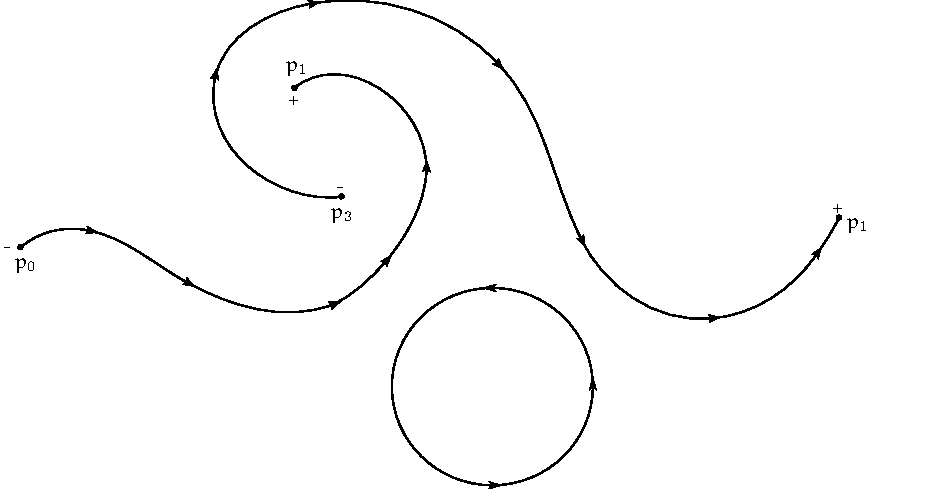
\includegraphics[width=.65\linewidth]{pics/chap10-1-o.pdf} 
  % \caption{}
  \label{fig:10-1}
\end{figure}

\begin{theorem}[Stokes' theorem]\label{theorem:10-8}\index{Stokes' Theorem}
  Let $N\sseq M^n$ be a domain with smooth boundary in an oriented smooth manifold. Let $\partial N$
  have induced orientation. For every $\omega\in\Omega^{n-1}(M)$ with $M\cap \supp_M(\omega)$ compact
  we have 
  \begin{align*}
    \int_{\partial N} i^*(\omega) = \int_N \dd\omega,
  \end{align*}
  where $i:\partial N\to M$ is the inclusion map.
\end{theorem}

\begin{proof}
  We assume that $n\ge 2$ and leave it to the reader to make the necessary
  changes for the case $n = 1$.

  It is clear that $i^*(\omega)$ has compact support. We can choose $f\in\Omega^0_c(M)$ with value
  constantly equal to 1 on $N\cap\supp_M(\omega)$. Since $f\omega$ coincides with $\omega$ on $N$, 
  both integrals are unchanged when $\omega$ is replaced by $f(\omega)$, so we may assume that $omega$
  has compact support.

  Choose a smooth atlas on $M$ consisting of charts of the type of Definition \ref{def:10-5}
  and a subordinate smooth partition of unity $(\rho\alpha)_{\alpha\in A}$. The formulas
  \begin{align*}
    \int_{\partial N}\omega = \sum_{\alpha} \int_{\partial N} 
    &&
    \int_N \dd\omega = \sum_{\alpha} \int_N \dd(\rho_\alpha\omega)
  \end{align*}

  reduce the problem to the case where $\omega\in\Omega^n_c(M)$. $\supp_M(\omega)\sseq U$
  and $(U, h)$ is a smooth chart $h(U\cap N) = h(U)\cap\RR^n_-$. Furthermore the chart $(U, h)$
  is assumed to be positively oriented.

  Let $\kappa\in\Omega^{n-1}_c(\RR^n)$ be the $(n-1)$-form that is $(h^{-1})^*(\omega)$ on 
  $h(U)$ and 0 on the rest of $\RR^n$. By diffeomorphism invariance we then have that 
  \begin{align*}
    \int_{\partial N}\omega 
      = \int_{h(U)\cap \partial\RR^n_-} (h^{-1})^*(\omega) 
      = \int_{\RR^n_-} \kappa
  \end{align*}
  and 
  \begin{align*}
    \int_N \dd\omega
      = \int_{h(U)\cap \RR^n_-} (h^{-1})^* \dd(\omega) 
      = \int_{\RR^n_-} \dd\kappa.
  \end{align*}
  Hence the proof reduces to the special case where $M=\RR^n, N=\RR^n_-$ and 
  $\omega\in\Omega_c^{n-1}(\RR^n)$. This case treated by direct calculation. We define 
  \begin{align*}
    \omega = \sum_{i=1}^{n }{f_i(x)\dd x_1\wedge\cdots\wedge\widehat{\dd x_i}\wedge\cdots\wedge\dd x_n},
  \end{align*}
  and choose $b>0$ such that $\supp_{\RR^n}f_i \sseq [-b, b]^n, 1\le i\le n$. Using Theorem \ref{theorem:3-12},
  \begin{align*}
    \omega_{|\partial\RR^n_-}
    = f_1(0, x_2, \cdots, x_n)\dd x_2\wedge\cdots\wedge\dd x_n.
  \end{align*}
  Hence 
  \begin{align}\label{eq:10-3}
    \int_{\partial\RR^n_-}\omega 
    = \int f_1(0, x_2, \cdots, x_n)\dd\mu_{n-1}.
  \end{align}
  By Theorem \ref{theorem:3-7} we have 
  \begin{align*}
    \dd\omega 
    = \sum_{i=1}^{n}{(-1)^{i-1}\frac{\partial f_i}{\partial x_i}\dd x_1\wedge\cdots\wedge\dd x_n}.
  \end{align*}
  Hence 
  \begin{align}\label{eq:10-4}
    \int_{\RR^n_-}
    = \sum_{i=1}^{n}{(-1)^{i-1}\int_{\RR^n_-}\frac{\partial f_i}{\partial x_i}\dd\mu_n}.
  \end{align}
  For $2\le i\le n$ we get 
  \begin{align*}
    & \int_{-\infty}^\infty \frac{\partial f_i}{\partial x_i}(x_1, \cdots, x_{i-1}, t, x_{i+1}, \cdots, x_n)\dd t \\
    = & f_i(x_1, \cdots, x_{i-1}, b, x_{i+1}, \cdots, x_n) 
      - f_i(x_1, \cdots, x_{i-1}, -b, x_{i+1}, \cdots, x_n).\\
    = & 0
  \end{align*}
  and then by Fubini's theorem
  \begin{align}\label{eq:10-5}
    \int_{\RR^n_-}\frac{\partial f_i}{\partial x_i}\dd\mu_n = 0\qquad (2\le i\le n).
  \end{align}
  When $i=1$, one gets 
  \begin{align*}
    \int_{-\infty}^0 \frac{\partial f_1}{\partial x_1}(t, x_2, \cdots, x_n)\dd t
    & = f_1(0, x_2, \cdots, x_n) - f_1(-b, x_2, \cdots, x_n)\\
    & = f_1(0, x_2, \cdots, x_n),
  \end{align*}
  and by Fubini's theorem 
  \begin{align}\label{eq:10-6}
    \int_{\RR^n_-} \frac{\partial f_1}{\partial x_1}\dd\mu_n
      = f_1(0, x_2, \cdots, x_n)\dd\mu_{n-1}.
  \end{align}
  By combining Equations \eqref{eq:10-3}--\eqref{eq:10-6} the desired formula follows.
\end{proof}

Taking $N = M$ in Theorem \ref{theorem:10-8} we have
\begin{corollary}\label{corollary:10-9}
  If $M^n$ is an oriented smooth manifold and $\omega\in\Omega^{n-1}_c(M)$ then 
  $\int_M\dd\omega=0$.
\end{corollary}

\begin{remark}\label{remark:10-10}
  Let $\omega$ be a closed $d$-form on $M^n$. One way of showing that the Cohomology class $[\omega]\in H^d(M)$
  is non-zero is to show that 
  \begin{align}\label{eq:10-7}
    \int_Q f^*(\omega) \neq 0
  \end{align}
  for a suitably chosen smooth map $f:Q^d\to M$ from a $d$-dimensional compact
  oriented smooth manifold $Q^d$. If $\omega=d\tau$ for some $\tau\in\Omega^{d-1}(M)$, then 
  Corollary \ref{corollary:10-9} yields
  \begin{align*}
    \int_Q f^*(\omega) = \int_Q \dd(f^*(\tau)) = 0.
  \end{align*}
  This, in essence, was the strategy from Examples \ref{example:1-2} and \ref{example:1-7}. It can 
  be shown (albeit in a very indirect way via cobordism theory) that $[\omega]=0$ if and only if
  all integrals of the form of \ref{eq:10-7} vanish.
\end{remark}


\begin{example}\label{example:10-11}
  In Example \ref{example:9-18} we considered the closed $(n -1)$-form on $\RR^n-\{0\}$,
  \begin{align*}
    \omega = \frac{1}{\|x\|^n} \sum_{i=1}^{n }{(-1)^{i-1}x_i\dd x_1\wedge\cdots\wedge\widehat{\dd x_i}\wedge\cdots\wedge\dd x_n}.
  \end{align*}
  Since the pre-image of $\omega$ under the inclusion of $S^{n-1}$ is the volume form $\R{vol}_{S^{n-1}}$,
  which has positive integral over $S^{n-1}$, we can conclude from Remark \ref{remark:10-10} that
  $[\omega]\neq 0$ in $H^{n-1} (\RR^n -\{0\})$. If $n\ge 2$ then, by Theorem \ref{theorem:6-13}, $[\omega]$ 
  is a basis of $H^{n-1} (\RR^n -\{0\})$. We thus have an isomorphism
  \begin{align*}
    H^{n-1} (\RR^n -\{0\})\simee \RR\qquad (n\ge 2)
  \end{align*}
  defined by integration over $S^{n-1}$. The image of $[\omega]$ under this isomorphism is
  the volume
  \begin{align*}
    \R{Vol}(S^{n-1}) = \int_{S^{n-1}} \R{vol}_{S^{n-1}}.
  \end{align*}
\end{example}

\begin{example}\label{example:10-12}
  The volume of $S^{n-1}$ can be calculated by applying Stokes' theorem to $D^n$ with the 
  standard orientation of IRn and the $(n - 1)$-fonn on $\RR^n$ given by
  \begin{align*}
    \omega_0 = \sum_{i=1}^{n}{(-1)^{i-1}x_i \dd x_1\wedge\cdots\wedge\widehat{\dd x_i}\wedge\cdots\wedge\dd x_n}.
  \end{align*}
  Since $\omega_{0|S^{n-1}} = \R{vol}_{S^{n-1}}$ and $\dd\omega_0 = n\dd x_1\wedge\cdots\wedge\dd x_n$ we have that 
  \begin{align*}
    \R{Vol}(S^{n-1}) 
    = \int_{S^{n-1}}\omega_0
    = \int_{D^n}\dd\omega_0
    = n\R{Vol}(D^n).
  \end{align*}
  By induction on $m$ and Fubini's theorem, it can be shown that
  \begin{align*}
    \R{Vol}(D^{2m}) = \frac{\pi^{m}}{m!}, && 
    \R{Vol}(D^{2m+1}) = \frac{2^{2m+1}m!\pi^{m}}{(2m+1)!}.
  \end{align*}
  This yields
  \begin{align*}
    \R{Vol}(S^{2m-1}) = \frac{2\pi^{m}}{(m-1)!}, &&
    \R{Vol}(S^{2m}) = \frac{2^{2m+1}m!\pi^{m}}{(2m)!}.
  \end{align*}
\end{example}

We conclude this chapter with a proof of the following:

\begin{theorem}\label{theorem:10-13}
  If $M^n$ is a connected oriented smooth manifold, then the sequence
  \begin{align}\label{eq:10-8}
    \Omega^{n-1}_c(M)
    \xra[\dd] \Omega^n_c(M)
    \xra[\int_M] \RR
    \xra 0
  \end{align}
  is exact.
\end{theorem}

\begin{corollary}\label{corollary:10-14}
  For a connected compact smooth manifold $M^n$, integration over $M$ induces an isomorphism
  \begin{align*}
    \int_M: H^n(M^n)\xra[\simee] \RR.\tag*{\qedsymbol}
  \end{align*}
\end{corollary}

In \eqref{eq:10-8} it is obvious that the integral is non-zero and hence surjective. It follows
from Corollary \ref{corollary:10-9} that the image of $\dd$ is contained in the kernel of the 
integral. We show the converse inclusion.

\begin{lemma}\label{lemma:10-15}
  Theorem \ref{theorem:10-13} holds for $M=\RR^n, n\ge 1$.
\end{lemma}

\begin{proof}
  Let $\omega\in\Omega^n_c(\RR^n)$ be a diffeomorphism $n$-form with $\int_{\RR^n}\omega=0$. We must find 
  that $\kappa\in\Omega^{n-1}_c(\RR^n)$, such that $\dd\kappa=\omega$. We can write $\omega=f(\FF{x})\dd x_1 \wedge\cdots\wedge\dd x_n$,
  and let 
  \begin{align*}
    \kappa = \sum_{j=1}^{n }{(-1)^{i-1}f_j(\FF{x})\dd x_1\wedge\cdots\wedge\widehat{\dd x_j}\wedge\cdots\wedge\dd x_n}. 
  \end{align*}
  A simple calculation gives 
  \begin{align*}
    \dd\kappa = \left(\sum_{j=1}^{n}{\frac{\partial f_j}{\partial x_j}}\right)\dd x_1\wedge\cdots\wedge\dd x_n.
  \end{align*}
  Hence we need to prove the following assertion:\par 
  ($P_n$): Let $f\in C_c^\infty(\RR^n)$ be a function with $\int f(x)\dd\mu_n = 0$. There exsits functions
  $f_1, \cdots, f_n$ in $C_c^\infty(\RR^n)$ such that
  \begin{align*}
    \sum_{j=1}^{n}{\frac{\partial f_j }{\partial x_j }} = f.
  \end{align*}
  We prove ($P_n$) by induction. For $n=1$ we are given a smooth function $x\in C_c^\infty(\RR)$ 
  with $\int_{-\infty}^\infty f(t)\dd t = 0$. The problem is solved by setting 
  \begin{align*}
    f_1(x) = \int_{-\infty}^x f(t)\dd t.
  \end{align*}
  Assume that ($P_{n-1}$) for $n\ge 2$, and let $f\in C_c^\infty(\RR^n, \RR)$ be a function with $\int f(x)\dd\mu_n = 0$.
  We choose $C>0$ with $\supp(f)\sseq [-C, C]^n$ and define 
  \begin{align}\label{eq:10-9}
    g(x_1, \cdots, x_{n-1}) = \int_{-\infty}^{\infty} f(x_1, \cdots, x_{n-1}, x_n)\dd x_n.
  \end{align}
  (The limits can be be replaced by $-C$ and $C$, respectively). The function $g$ is smooth, 
  since we can differentiate under the integral sign. Furthennore $\supp(g)\sseq [-C, C]^{n-1}$. 
  Fubini's theorem yields $\int g\dd\mu_{n-1} = \int f\dd\mu_n = 0$. Using $(P_{n-1})$ we get functions 
  $g_1, \cdots, g_{n-1}$ in $C_c^\infty(\RR^{n-1}, \RR)$ with 
  \begin{align}\label{eq:10-10}
    \sum_{j=1}^{n-1}{\frac{\partial g_j}{\partial x_j}} = g.
  \end{align}
  We choose a function $\rho\in C_c^\infty(\RR, \RR)$ with $\int_{-\infty}^\infty \rho(t)\dd t = 1$, and 
  define $f_j\in C_c^\infty(\RR^n, \RR)$,
  \begin{align}\label{eq:10-11}
    f_j(x_1, \cdots, x_n) = g_j(x_1, \cdots, x_{n-1})\rho(x_n), 1\le j\le n-1.
  \end{align}
  Let $h\in C_c^\infty(\RR, \RR)$ be the function
  \begin{align}\label{eq:10-12}
    h = f - \sum_{j=1}^{n-1}{\frac{\partial f_j}{\partial x_j}}.
  \end{align}
  A function $f_n \in C_c^\infty(\RR^n)$ with $\partial f_n/\partial x_n=h$ is given by
  \begin{align}\label{eq:10-13}
    f_n(x_1, \cdots, x_{n-1}, x_n) = \int_{-\infty}^{x_n} h(x_1, \cdots, x_{n-1}, t)\dd t.
  \end{align}

  It is obvious that $f_n$ is smooth, but we must show that it has compact support. To
  this end it is sufficient to show that the integral of \eqref{eq:10-13} vanishes when the upper
  limit X n is replaced by 00. Now \eqref{eq:10-10}, \eqref{eq:10-11} and \eqref{eq:10-12} yield 
  that
  \begin{align*}
    h(x_1, \cdots, x_{n-1}, x_n) 
    & = f(x_1, \cdots, x_{n-1}, t) - \sum_{j=1}^{n-1}{\frac{\partial g_j}{\partial x_j}}\rho(t)\\
    & = f(x_1, \cdots, x_{n-1}, t) - g(x_1, \cdots, x_{n-1})\rho(t).
  \end{align*}
  Finally from \eqref{eq:10-10} it follows that 
  \begin{align*}
    & \int_{-\infty}^\infty h(x_1, \cdots, x_{n-1}, t)\dd t \\
    = & \int_{-\infty}^\infty f(x_1, \cdots, x_{n-1}, t)\dd t 
      - g(x_1, \cdots, x_{n-1})\int_{-\infty}^\infty \rho(t)\dd t\\
    = & 0.
  \end{align*}
\end{proof}

\begin{lemma}\label{lemma:10-16}
  Let $(U_\alpha)_{\alpha\in A}$ be an open cover of the connected manifold $M$, and 
  let $p, q\in M$. There exists indices $\alpha_1, \cdots, \alpha_k$ such that 
  \begin{enumerate}[(i)]
    \item $p\in U_\alpha$ and $q\in U_{\alpha_k}$.
    \item $U_{\alpha_i}\cap U_{\alpha_{i+1}}\neq\ns$ for $1\le i\le k-1$.
  \end{enumerate}
\end{lemma}

\begin{proof}
  For a fixed $p$ we define $V$ to be the set of $q\in M$, for which there exists
a finite sequence of indices $\alpha_1, \cdots, \alpha_k$ from $A$, such that (i) and (ii) are 
satisfied. It is obvious that $V$ is both open and closed in $M$ and that $V$ contains $p$. Since
$M$ is connected, we must have $V = M$.
\end{proof}

\begin{lemma}\label{lemma:10-17}
  Let $U\sseq M$ be an open set diffeomorphic to $\RR^n$ and let $W\sseq U$ be 
  non-empty and open. For every $\omega\in\Omega^n_c(M)$ with $\supp_M(\omega)\sseq U$, there 
  exists a $\kappa\in\Omega^{n-1}_c(M)$ such that $\supp\kappa\sseq U$ and $\supp(\omega-\dd\kappa)\sseq W$.
\end{lemma}

\begin{proof}
  It suffices to prove the lemma when $M = U$, and by diffeomorphism
invariance it is enough to consider the case where $M = U = \RR^n$. Choose $\omega_1\in\Omega_c^n(\RR^n)$
with $\supp(\omega_1)\sseq W$ and $\int_{\RR^n}\omega_1 = 1$. Then 
\begin{align*}
  \int_{\RR^n} (\omega -a\omega_1) = 0, \qquad \text{ where } a = \int_{\RR^n}\omega.
\end{align*}

By Lemma \ref{lemma:10-15} we can find a $\kappa\in\Omega^{n-1}_c(\RR^n)$ with 
\begin{align*}
  \omega - a\omega_1 = \dd\kappa.
\end{align*}
Hence $\omega - \dd\kappa = \dd\omega_1$ has its support in $W$.
\end{proof}

\begin{lemma}\label{lemma:10-18}
  Assume that $M^n$ is connected and let $W\sseq M$ be non-empty and 
  open. For every $\omega\in\Omega^n_c(M)$ there exists a $\kappa\in\Omega^{n-1}_c(M)$ with 
  $\supp(\omega-\dd\kappa)\sseq W$.
\end{lemma}

\begin{proof}
  Suppose that $\supp\omega\sseq U_1$ for some open set $U_1\sseq M$ diffeomorphic to 
  $\RR^n$. We apply Lemma \ref{lemma:10-16} to find open sets $U_2, \cdots, U_k$, diffeomorphic 
  to $\RR^n$, such that $U_{i-1}\cap U_i\neq \ns$ for $2\le i\le k$ and $U_k\sseq W$. We use Lemma 
  \ref{lemma:10-17} to successively choose $\kappa_1, \cdots, \kappa_{k-1}$ in $\Omega^{n-1}_c(M)$ such that 
  \begin{align*}
    \supp\left(\omega - \sum_{i=1}^{j }{\dd\kappa_i }\right)
    \sseq U_j\cap U_{j+1}\qquad (1\le j\le k-1).
  \end{align*}

  The lemma holds for $\kappa = \sum_{i=1}^{k-1}{\kappa_i}$.

  In the general case we use a partition of unity to write
  \begin{align*}
    \omega = \sum_{j = 1}^{m }{\omega_j},
  \end{align*}
  where $\omega_j\in\Omega^n_c(M)$ has support contained in a open set diffeomorphic to $\RR^n$. 
  The above gives $\tilde{\kappa}_j\in\Omega^{n-1}_c(M), 1\le j\le m$, such that $\supp(\omega_j-\dd\tilde{\kappa_j})\sseq W$.
  For 
  \begin{align*}
    \tilde{\kappa} = \sum_{j=1}^{m }{\tilde{\kappa}_j} \in \Omega^{n-1}_c(M)
  \end{align*}
  we have that
  \begin{align*}
    \omega -\dd\tilde{\kappa} = \sum_{j=1}^{m }{(\omega_j - \dd\tilde{\kappa}_j)}
  \end{align*}
  Hence $\supp(\omega-\dd\tilde{\kappa})\sseq \cup_{j=1}^m\sseq W$.
\end{proof}

\textbf{Proof of Theorem \ref{theorem:10-13}.} Suppose given $\omega\in\Omega^n_c(M)$ with 
$\int_M\omega = 0$. Choose an open set $W\sseq M$ diffeomorphic to $\RR^n$. By Lemma \ref{lemma:10-18}
we can find a $\kappa\in\Omega_c^{n-1}\sseq W$. But then by Corollary \ref{corollary:10-9},
\begin{align*}
  \int_W (\omega - \dd\kappa) 
  = \int_M (\omega - \dd\kappa)
  = - \int_M\dd\kappa 
  = 0
\end{align*}

Lemma \ref{lemma:10-15} implies that Theorem \ref{theorem:10-13} holds for $W$, i.e. there 
exists a $\tau_0\in\Omega^{n-1}_c(W)$ that satisfies
\begin{align*}
  (\omega - \dd\kappa)_{|W} = \dd\tau_0.
\end{align*}

Let $\tau\in \Omega^{n-1}_c(M)$ be the extension of $\tau_0$ which vanishes outside $\supp_W(\tau_0)$.
Then $\omega -\dd\kappa=\dd\tau$, so $\tau+\kappa$ maps $\omega$ under $d$. \hfill\(\qedsymbol\)